%  LaTeX support: latex@mdpi.com 
%  For support, please attach all files needed for compiling as well as the log file, and specify your operating system, LaTeX version, and LaTeX editor.

%=================================================================
\documentclass[journal,article,submit,pdftex,moreauthors]{Definitions/mdpi} 
%\documentclass[preprints,article,submit,pdftex,moreauthors]{Definitions/mdpi} 
% For posting an early version of this manuscript as a preprint, you may use "preprints" as the journal. Changing "submit" to "accept" before posting will remove line numbers.

% Below journals will use APA reference format:
% admsci, aieduc, behavsci, businesses, econometrics, economies, education, ejihpe, famsci, games, humans, ijcs, ijfs, journalmedia, jrfm, languages, psycholint, publications, tourismhosp, youth

% Below journals will use Chicago reference format:
% arts, genealogy, histories, humanities, jintelligence, laws, literature, religions, risks, socsci

%--------------------
% Class Options:
%--------------------
%----------
% journal
%----------
% Choose between the following MDPI journals:
% accountaudit, acoustics, actuators, addictions, adhesives, admsci, adolescents, aerobiology, aerospace, agriculture, agriengineering, agrochemicals, agronomy, ai, air, algorithms, allergies, alloys, amh, analytica, analytics, anatomia, anesthres, animals, antibiotics, antibodies, antioxidants, applbiosci, appliedchem, appliedmath, appliedphys, applmech, applmicrobiol, applnano, applsci, aquacj, architecture, arm, arthropoda, arts, asc, asi, astronomy, atmosphere, atoms, audiolres, automation, axioms, bacteria, batteries, bdcc, behavsci, beverages, biochem, bioengineering, biologics, biology, biomass, biomechanics, biomed, biomedicines, biomedinformatics, biomimetics, biomolecules, biophysica, biosensors, biosphere, biotech, birds, blockchains, bloods, blsf, brainsci, breath, buildings, businesses, cancers, carbon, cardiogenetics, catalysts, cells, ceramics, challenges, chemengineering, chemistry, chemosensors, chemproc, children, chips, cimb, civileng, cleantechnol, climate, clinbioenerg, clinpract, clockssleep, cmd, cmtr, coasts, coatings, colloids, colorants, commodities, complications, compounds, computation, computers, condensedmatter, conservation, constrmater, cosmetics, covid, crops, cryo, cryptography, crystals, csmf, ctn, curroncol, cyber, dairy, data, ddc, dentistry, dermato, dermatopathology, designs, devices, diabetology, diagnostics, dietetics, digital, disabilities, diseases, diversity, dna, drones, dynamics, earth, ebj, ecm, ecologies, econometrics, economies, education, eesp, ejihpe, electricity, electrochem, electronicmat, electronics, encyclopedia, endocrines, energies, eng, engproc, ent, entomology, entropy, environments, epidemiologia, epigenomes, esa, est, famsci, fermentation, fibers, fintech, fire, fishes, fluids, foods, forecasting, forensicsci, forests, fossstud, foundations, fractalfract, fuels, future, futureinternet, futureparasites, futurepharmacol, futurephys, futuretransp, galaxies, games, gases, gastroent, gastrointestdisord, gastronomy, gels, genealogy, genes, geographies, geohazards, geomatics, geometry, geosciences, geotechnics, geriatrics, glacies, grasses, greenhealth, gucdd, hardware, hazardousmatters, healthcare, hearts, hemato, hematolrep, heritage, higheredu, highthroughput, histories, horticulturae, hospitals, humanities, humans, hydrobiology, hydrogen, hydrology, hygiene, idr, iic, ijerph, ijfs, ijgi, ijmd, ijms, ijns, ijpb, ijt, ijtm, ijtpp, ime, immuno, informatics, information, infrastructures, inorganics, insects, instruments, inventions, iot, j, jal, jcdd, jcm, jcp, jcs, jcto, jdad, jdb, jeta, jfb, jfmk, jimaging, jintelligence, jlpea, jmahp, jmmp, jmms, jmp, jmse, jne, jnt, jof, joitmc, joma, jop, jor, journalmedia, jox, jpbi, jpm, jrfm, jsan, jtaer, jvd, jzbg, kidney, kidneydial, kinasesphosphatases, knowledge, labmed, laboratories, land, languages, laws, life, lights, limnolrev, lipidology, liquids, literature, livers, logics, logistics, lubricants, lymphatics, machines, macromol, magnetism, magnetochemistry, make, marinedrugs, materials, materproc, mathematics, mca, measurements, medicina, medicines, medsci, membranes, merits, metabolites, metals, meteorology, methane, metrics, metrology, micro, microarrays, microbiolres, microelectronics, micromachines, microorganisms, microplastics, microwave, minerals, mining, mmphys, modelling, molbank, molecules, mps, msf, mti, multimedia, muscles, nanoenergyadv, nanomanufacturing, nanomaterials, ncrna, ndt, network, neuroglia, neurolint, neurosci, nitrogen, notspecified, nursrep, nutraceuticals, nutrients, obesities, oceans, ohbm, onco, oncopathology, optics, oral, organics, organoids, osteology, oxygen, parasites, parasitologia, particles, pathogens, pathophysiology, pediatrrep, pets, pharmaceuticals, pharmaceutics, pharmacoepidemiology, pharmacy, philosophies, photochem, photonics, phycology, physchem, physics, physiologia, plants, plasma, platforms, pollutants, polymers, polysaccharides, populations, poultry, powders, preprints, proceedings, processes, prosthesis, proteomes, psf, psych, psychiatryint, psychoactives, psycholint, publications, purification, quantumrep, quaternary, qubs, radiation, reactions, realestate, receptors, recycling, regeneration, religions, remotesensing, reports, reprodmed, resources, rheumato, risks, robotics, rsee, ruminants, safety, sci, scipharm, sclerosis, seeds, sensors, separations, sexes, signals, sinusitis, siuj, skins, smartcities, sna, societies, socsci, software, soilsystems, solar, solids, spectroscj, sports, standards, stats, std, stresses, surfaces, surgeries, suschem, sustainability, symmetry, synbio, systems, tae, targets, taxonomy, technologies, telecom, test, textiles, thalassrep, therapeutics, thermo, timespace, tomography, tourismhosp, toxics, toxins, transplantology, transportation, traumacare, traumas, tropicalmed, universe, urbansci, uro, vaccines, vehicles, venereology, vetsci, vibration, virtualworlds, viruses, vision, waste, water, wem, wevj, wild, wind, women, world, youth, zoonoticdis

%---------
% article
%---------
% The default type of manuscript is "article", but can be replaced by: 
% abstract, addendum, article, benchmark, book, bookreview, briefcommunication, briefreport, casereport, changes, clinicopathologicalchallenge, comment, commentary, communication, conceptpaper, conferenceproceedings, correction, conferencereport, creative, datadescriptor, discussion, entry, expressionofconcern, extendedabstract, editorial, essay, erratum, fieldguide, hypothesis, interestingimages, letter, meetingreport, monograph, newbookreceived, obituary, opinion, proceedingpaper, projectreport, reply, retraction, review, perspective, protocol, shortnote, studyprotocol, supfile, systematicreview, technicalnote, viewpoint, guidelines, registeredreport, tutorial,  giantsinurology, urologyaroundtheworld
% supfile = supplementary materials

%----------
% submit
%----------
% The class option "submit" will be changed to "accept" by the Editorial Office when the paper is accepted. This will only make changes to the frontpage (e.g., the logo of the journal will get visible), the headings, and the copyright information. Also, line numbering will be removed. Journal info and pagination for accepted papers will also be assigned by the Editorial Office.

%------------------
% moreauthors
%------------------
% If there is only one author the class option oneauthor should be used. Otherwise use the class option moreauthors.

%---------
% pdftex
%---------
% The option pdftex is for use with pdfLaTeX. Remove "pdftex" for (1) compiling with LaTeX & dvi2pdf (if eps figures are used) or for (2) compiling with XeLaTeX.

%=================================================================
% MDPI internal commands - do not modify
\firstpage{1} 
\makeatletter 
\setcounter{page}{\@firstpage} 
\makeatother
\pubvolume{1}
\issuenum{1}
\articlenumber{0}
\pubyear{2025}
\copyrightyear{2025}
%\externaleditor{Firstname Lastname} % More than 1 editor, please add `` and '' before the last editor name
\datereceived{ } 
\daterevised{ } % Comment out if no revised date
\dateaccepted{ } 
\datepublished{ } 
%\datecorrected{} % For corrected papers: "Corrected: XXX" date in the original paper.
%\dateretracted{} % For retracted papers: "Retracted: XXX" date in the original paper.
\hreflink{https://doi.org/} % If needed use \linebreak
%\doinum{}
%\pdfoutput=1 % Uncommented for upload to arXiv.org
%\CorrStatement{yes}  % For updates
%\longauthorlist{yes} % For many authors that exceed the left citation part

%=================================================================
% Add packages and commands here. The following packages are loaded in our class file: fontenc, inputenc, calc, indentfirst, fancyhdr, graphicx, epstopdf, lastpage, ifthen, float, amsmath, amssymb, lineno, setspace, enumitem, mathpazo, booktabs, titlesec, etoolbox, tabto, xcolor, colortbl, soul, multirow, microtype, tikz, totcount, changepage, attrib, upgreek, array, tabularx, pbox, ragged2e, tocloft, marginnote, marginfix, enotez, amsthm, natbib, hyperref, cleveref, scrextend, url, geometry, newfloat, caption, draftwatermark, seqsplit
% cleveref: load \crefname definitions after \begin{document}

%=================================================================
% Please use the following mathematics environments: Theorem, Lemma, Corollary, Proposition, Characterization, Property, Problem, Example, ExamplesandDefinitions, Hypothesis, Remark, Definition, Notation, Assumption
%% For proofs, please use the proof environment (the amsthm package is loaded by the MDPI class).

%=================================================================
% Full title of the paper (Capitalized)
\Title{Design and Implementation of a UART Module on FPGA Using RTL for Cryptographic Encryption and Decryption Techniques}

% MDPI internal command: Title for citation in the left column
\TitleCitation{Title}

% Author Orchid ID: enter ID or remove command
\newcommand{\orcidauthorA}{0000-0000-0000-000X} % Add \orcidA{} behind the author's name
%\newcommand{\orcidauthorB}{0000-0000-0000-000X} % Add \orcidB{} behind the author's name

% Authors, for the paper (add full first names)
\Author{Christian-Antonio Colin-Cejudo$^{1,\dagger,\ddagger}$\orcidA{}, Gonzalo-Issac Duchén-Sánchez $^{2,\ddagger}$ and Gabriel Sánchez-Pérez $^{3,\dagger}$}

%\longauthorlist{yes}

% MDPI internal command: Authors, for metadata in PDF
\AuthorNames{Firstname Lastname, Firstname Lastname and Firstname Lastname}

% MDPI internal command: Authors, for citation in the left column, only choose below one of them according to the journal style
% If this is a Chicago style journal 
% (arts, genealogy, histories, humanities, jintelligence, laws, literature, religions, risks, socsci): 
% Lastname, Firstname, Firstname Lastname, and Firstname Lastname.

% If this is a APA style journal 
% (admsci, behavsci, businesses, econometrics, economies, education, ejihpe, games, humans, ijfs, journalmedia, jrfm, languages, psycholint, publications, tourismhosp, youth): 
% Lastname, F., Lastname, F., \& Lastname, F.

% If this is a ACS style journal (Except for the above Chicago and APA journals, all others are in the ACS format): 
% Lastname, F.; Lastname, F.; Lastname, F.
\isAPAStyle{%
       \AuthorCitation{Lastname, F., Lastname, F., \& Lastname, F.}
         }{%
        \isChicagoStyle{%
        \AuthorCitation{Lastname, Firstname, Firstname Lastname, and Firstname Lastname.}
        }{
        \AuthorCitation{Lastname, F.; Lastname, F.; Lastname, F.}
        }
}

% Affiliations / Addresses (Add [1] after \address if there is only one affiliation.)
\address{%
$^{1}$ \quad Affiliation 1; christian.upiita@gmai.com\\
$^{2}$ \quad Affiliation 2; gduchen@ieee.org\\
$^{3}$ \quad Affiliation 3; caaann@gmail.com}
% Contact information of the corresponding author
\corres{Correspondence: e-mail@e-mail.com; Tel.: (optional; include country code; if there are multiple corresponding authors, add author initials) +xx-xxxx-xxx-xxxx (F.L.)}

% Current address and/or shared authorship
\firstnote{Current address: Affiliation.}  % Current address should not be the same as any items in the Affiliation section.
\secondnote{These authors contributed equally to this work.}
% The commands \thirdnote{} till \eighthnote{} are available for further notes

%\simplesumm{} % Simple summary

%\conference{} % An extended version of a conference paper

% Abstract (Do not insert blank lines, i.e. \\) 
\abstract{The increasing demand for robust and efficient information security has led to the growing adoption of specialized hardware for cryptographic operations. In response to the rise in cyber threats and the need to process large volumes of data in real time, hardware-based cryptographic solutions offer significant advantages in terms of performance, resistance to attacks, and secure storage of cryptographic keys. This thesis presents the implementation of a secure communication system using the UART (Universal Asynchronous Receiver-Transmitter) protocol as the foundation for a Register Transfer Level (RTL) design on an FPGA platform. The base protocol was modified to introduce an additional hardware-level security layer. Furthermore, cryptographic techniques—specifically encryption and decryption—were integrated into the design to enhance data protection and integrity during transmission. The results demonstrate the feasibility of embedding cryptographic mechanisms directly into communication hardware, providing a scalable and efficient solution for secure embedded systems.}

% Keywords
\keyword{Cryptographic hardware; Information security; Encryption, Decryption; Cryptographic keys; Digital signatures; Authentication; Cyber threats; Data processing; Communication protocols; UART (Universal Asynchronous Receiver-Transmitter); FPGA (Field-Programmable Gate Array); RTL design (Register Transfer Level); Hardware security layer; Cryptographic techniques; Critical infrastructure.} 

% The fields PACS, MSC, and JEL may be left empty or commented out if not applicable
%\PACS{J0101}
%\MSC{}
%\JEL{}

%%%%%%%%%%%%%%%%%%%%%%%%%%%%%%%%%%%%%%%%%%
% Only for the journal Diversity
%\LSID{\url{http://}}

%%%%%%%%%%%%%%%%%%%%%%%%%%%%%%%%%%%%%%%%%%
% Only for the journal Applied Sciences
%\featuredapplication{Authors are encouraged to provide a concise description of the specific application or a potential application of the work. This section is not mandatory.}
%%%%%%%%%%%%%%%%%%%%%%%%%%%%%%%%%%%%%%%%%%

%%%%%%%%%%%%%%%%%%%%%%%%%%%%%%%%%%%%%%%%%%
% Only for the journal Data
%\dataset{DOI number or link to the deposited data set if the data set is published separately. If the data set shall be published as a supplement to this paper, this field will be filled by the journal editors. In this case, please submit the data set as a supplement.}
%\datasetlicense{License under which the data set is made available (CC0, CC-BY, CC-BY-SA, CC-BY-NC, etc.)}

%%%%%%%%%%%%%%%%%%%%%%%%%%%%%%%%%%%%%%%%%%
% Only for the journal BioTech, Fishes, Neuroimaging and Toxins
%\keycontribution{The breakthroughs or highlights of the manuscript. Authors can write one or two sentences to describe the most important part of the paper.}

%%%%%%%%%%%%%%%%%%%%%%%%%%%%%%%%%%%%%%%%%%
% Only for the journal Encyclopedia
%\encyclopediadef{For entry manuscripts only: please provide a brief overview of the entry title instead of an abstract.}

%%%%%%%%%%%%%%%%%%%%%%%%%%%%%%%%%%%%%%%%%%
% Only for the journal Advances in Respiratory Medicine, Future, Sensors and Smart Cities
%\addhighlights{yes}
%\renewcommand{\addhighlights}{%
%
%\noindent This is an obligatory section in ``Advances in Respiratory Medicine'', ``Future'', ``Sensors'' and ``Smart Cities”, whose goal is to increase the discoverability and readability of the article via search engines and other scholars. Highlights should not be a copy of the abstract, but a simple text allowing the reader to quickly and simplified find out what the article is about and what can be cited from it. Each of these parts should be devoted up to 2~bullet points.\vspace{3pt}\\
%\textbf{What are the main findings?}
% \begin{itemize}[labelsep=2.5mm,topsep=-3pt]
% \item First bullet.
% \item Second bullet.
% \end{itemize}\vspace{3pt}
%\textbf{What is the implication of the main finding?}
% \begin{itemize}[labelsep=2.5mm,topsep=-3pt]
% \item First bullet.
% \item Second bullet.
% \end{itemize}
%}

%%%%%%%%%%%%%%%%%%%%%%%%%%%%%%%%%%%%%%%%%%
\begin{document}

%%%%%%%%%%%%%%%%%%%%%%%%%%%%%%%%%%%%%%%%%%
\setcounter{section}{0} %% Remove this when starting to work on the template.
%\section{How to Use this Template}


% The order of the section titles is different for some journals. Please refer to the "Instructions for Authors” on the journal homepage.

\section{Introduction}

Currently, information security has become a fundamental pillar for the development of reliable digital systems. The increasing sophistication of cyber threats, combined with the exponential growth in data generation and transmission, demands increasingly robust and efficient solutions. In this context, the use of specialized hardware for cryptographic operations has emerged as an effective alternative to the limitations of software-only cryptographic processing.

Cryptographic hardware offers significant advantages, such as higher performance, lower latency, reduced energy consumption, and greater resistance to both physical and logical attacks. These characteristics make it an ideal solution for embedded systems, IoT devices, industrial applications, and environments where security and operational efficiency are top priorities.

Field Programmable Gate Arrays (FPGAs) have become one of the most versatile technologies for electronic system design. These devices provide a cost-effective solution, especially for low-volume production, since the initial cost of prototyping is considerably lower compared to Application-Specific Integrated Circuits (ASICs). Moreover, a key advantage is their reconfigurability during operation, which allows a single device to perform multiple predefined functions, thereby optimizing space and reducing costs.

Today, electronic systems are present in almost every aspect of daily life, from consumer products to industrial control systems, automotive applications, security, and beyond. The current trend in electronic design is characterized by the increasing complexity of components, which demands solutions that are user-friendly, versatile, low-power, and quick to market. Modern integrated circuit technology makes it possible to integrate these complex systems into highly compact dimensions, referred to as embedded systems or Systems on Chip (SoC). These systems, designed to fulfill specific functions, combine hardware and software tailored for each task. In this context, FPGAs, thanks to their reconfigurability, are valuable tools for developing prototypes or small-scale series at affordable costs.

Among the most widely used communication protocols in embedded systems is the Universal Asynchronous Receiver-Transmitter (UART), due to its simplicity, low implementation cost, and broad compatibility. However, this protocol lacks native security mechanisms, making it vulnerable to interception, manipulation, and unauthorized access.

This thesis proposes the design and implementation of a cryptographic security layer on top of the UART protocol, using a Register Transfer Level (RTL) approach on an FPGA platform. The implementation leverages a Hardware Description Language (HDL) to model and design digital circuits. The modification of the protocol not only ensures secure data transmission but also integrates encryption and decryption techniques directly into hardware. This solution aims to demonstrate the feasibility of incorporating efficient cryptographic security into embedded communication systems without compromising performance or scalability. 

%%%%%%%%%%%%%%%%%%%%%%%%%%%%%%%%%%%%%%%%%%
\section{Materials and Methods}

This chapter reviewed the foundations of classical cryptography, emphasizing the Caesar cipher as an illustrative example of monoalphabetic substitution techniques. While obsolete for modern applications due to its vulnerability to brute-force and frequency analysis attacks, the Caesar cipher remains valuable for educational purposes and as a test case for implementing sequential processing, finite state machines, and resource evaluation in FPGA-based platforms. Its simplicity makes it an effective starting point for understanding the relationship between mathematical algorithms and their hardware representation.

\subsection{Operation of the Algorithm}
From a mathematical perspective, the Caesar cipher can be represented by the following function:
\centerline{\(C(x) = ( x + k ) mod n \)}

Where:

\begin{itemize}
\item $C(x)$ is the encrypted character.
\item $x$ is the index of the character in the alphabet $A = 0, B = 1, \dots, Z = 25$.
\item $k$ is the shift key.
\item $n$ is the total number of characters in the alphabet, usually $n = 26$ for the Latin alphabet.
\end{itemize}

Decryption consists of applying the inverse operation:

\centerline{$P(x) = ( x - k ) \bmod n $}

For example, if the word \textbf{\textit{“HOLA”}} is encrypted with a shift of $k = 3$, the result is \textbf{\textit{“KROD”}}. To decrypt, the inverse shift is applied.


The discussion then traced the evolution of digital design methodologies, from early breadboard prototyping to the integration of computer-aided design (CAD) tools, which enabled accurate simulation and validation of electronic systems. The emergence of hardware description languages (HDL) such as VHDL and Verilog marked a turning point by providing standardized, structured methods for system modeling and verification. The subsequent development of SystemVerilog extended these capabilities, incorporating object-oriented programming, functional verification, and reusable testbench environments, thus consolidating the design and verification process within a unified framework.

A comparative analysis with software engineering highlighted both syntactic similarities and conceptual differences, underlining the importance of adopting a hardware-oriented mindset when aiming for physical synthesis and implementation on FPGA or ASIC platforms. This distinction is essential to ensure that HDL-based models accurately reflect hardware behavior rather than abstract algorithmic processes.

Finally, the Altera DE2-115 development board was presented as a versatile and widely adopted prototyping platform. Equipped with a Cyclone IV FPGA, embedded and external memories, extensive I/O interfaces, and compatibility with tools such as Quartus Prime, this board provides the necessary infrastructure for developing, simulating, and validating digital systems. Its relevance in academic and research contexts makes it particularly suitable for projects focused on integrating cryptographic algorithms into reconfigurable hardware architectures.





%%%%%%%%%%%%%%%%%%%%%%%%%%%%%%%%%%%%%%%%%%
\section{Results}

In order to validate the proposed obfuscation mechanism as an enhancement to the traditional Caesar cipher, a series of experiments were conducted both in software and hardware domains. The primary objective was to demonstrate that the integration of an additional obfuscation layer not only increases the complexity of deciphering the encrypted message but also preserves functional equivalence between the software prototype and its hardware implementation.

The first stage of the experimentation involved the development of a Python script that implemented the Caesar cipher combined with the proposed obfuscation technique. This environment allowed rapid prototyping and verification of functional correctness. Various input datasets, including alphanumeric strings and binary sequences, were subjected to encryption and decryption tests. Statistical measures were then applied to evaluate the distribution of ciphertext characters Fig. \ref{fig1}, aiming to confirm that the obfuscation achieved a reduction in predictable frequency patterns typically exploitable in classical substitution ciphers. The resulting charts demonstrated a noticeable flattening of character frequency distributions, indicating that the modified cipher effectively mitigates one of the main weaknesses of the traditional Caesar scheme.

\begin{figure}[H]
%\isPreprints{\centering}{} % Only used for preprints
%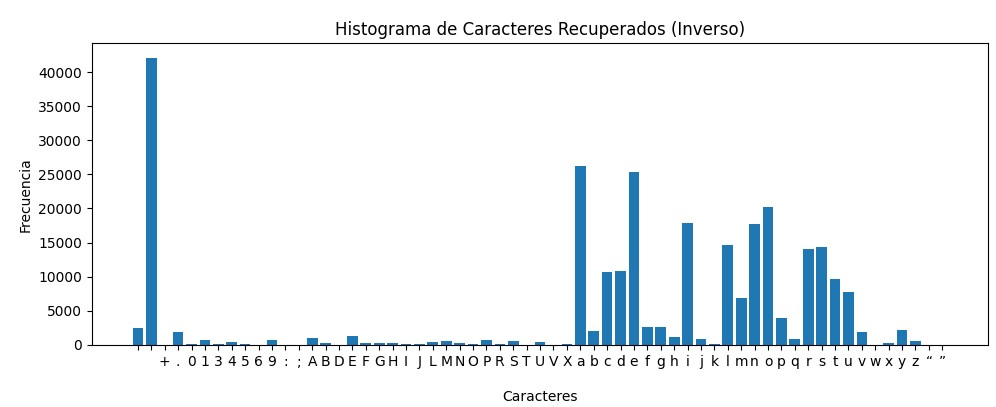
\includegraphics[width=4 cm]{imagenes/img1}
 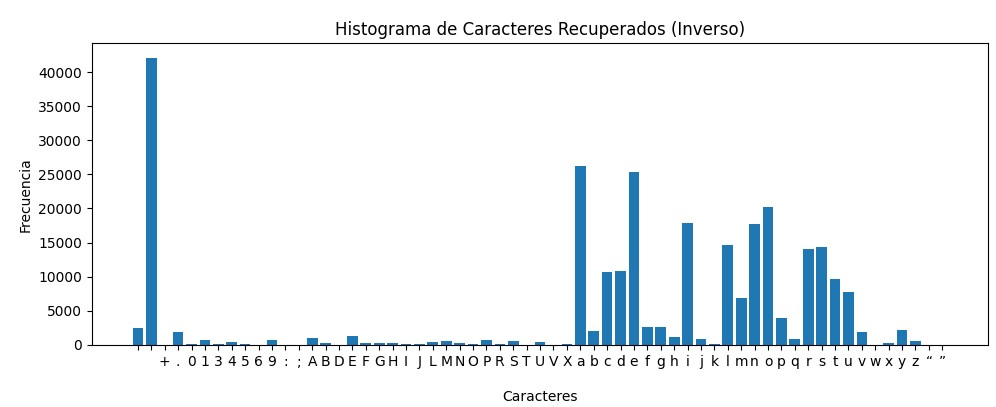
\includegraphics[width=1\textwidth, height=5 cm]{imagenes/img1} % Reemplaza con el nombre de tu archivo de imagen
\caption{Plain Spanish text distribution.\label{fig1}}
\end{figure}   
\unskip


Following successful validation in the software domain, the algorithm was translated into a hardware description suitable for FPGA implementation. Specifically, an RTL (Register Transfer Level) block was designed using VHDL to replicate the operations of both the Caesar cipher and the obfuscation layer. The choice of RTL ensured that the design remained synthesizable and could be physically deployed on the Altera DE2-115 FPGA platform. This translation process required special attention to timing, resource utilization, and concurrency management, as hardware execution introduces constraints not present in sequential software execution.

Simulation of the RTL block was performed prior to synthesis, ensuring that the output matched the reference Python implementation across all test vectors. Waveform analysis confirmed correct alignment of data paths, clock synchronization, and control logic behavior. Subsequently, the design was synthesized, placed, and routed onto the FPGA. Resource utilization reports indicated that the additional obfuscation logic introduced only a modest increase in logic element consumption, remaining well within the capacity of the Cyclone IV device.

To further validate the effectiveness of the hardware design, experimental results were collected directly from the FPGA implementation. Input text sequences were encrypted, processed through the obfuscation mechanism, and then decrypted in real time. The resulting ciphertexts were again subjected to statistical frequency analysis Fig. \ref{fig2}. Comparison between the software-generated and hardware-generated distributions confirmed functional equivalence: both platforms achieved similar levels of character dispersion and unpredictability.


\begin{figure}[H]
%\isPreprints{\centering}{} % Only used for preprints
%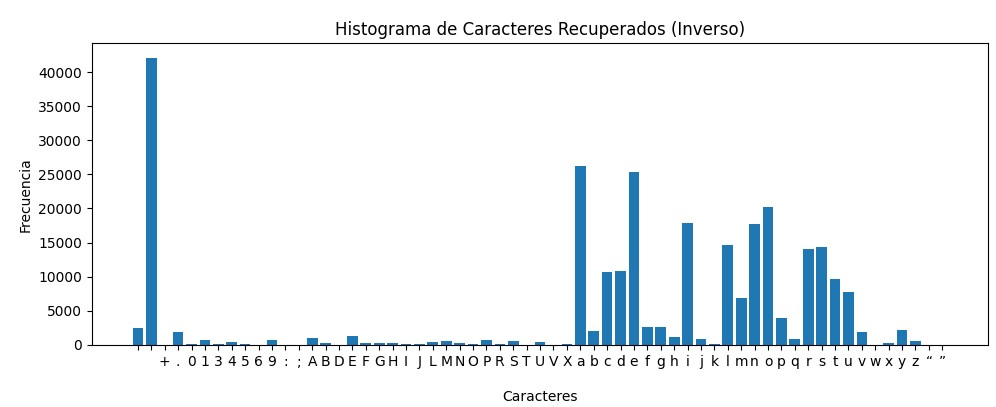
\includegraphics[width=4 cm]{imagenes/img1}
 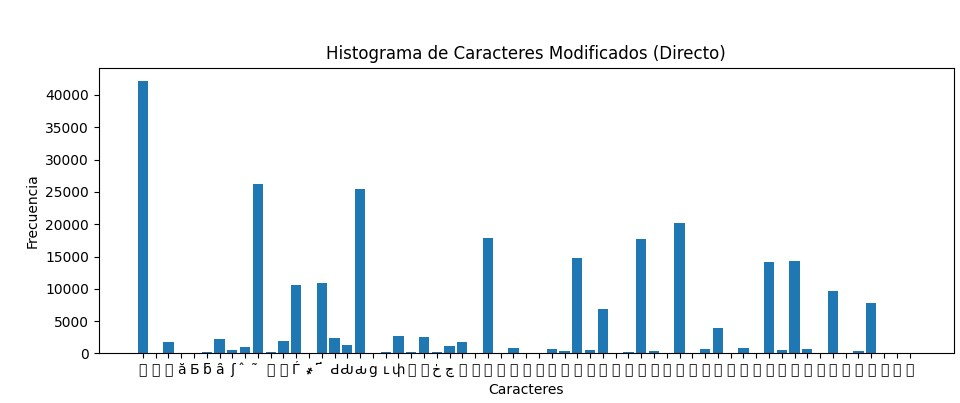
\includegraphics[width=1\textwidth, height=5 cm]{imagenes/img2} % Reemplaza con el nombre de tu archivo de imagen
\caption{Exit text hardware-generated obfuscation distribution.\label{fig2}}
\end{figure}   
\unskip

In summary, the experimental results provide strong evidence that the proposed obfuscation technique enhances the Caesar cipher without compromising its functional reliability. The consistency observed between the Python prototype and the FPGA-based RTL implementation demonstrates that the approach is both feasible and scalable across computational platforms. Furthermore, the low hardware resource overhead highlights the practicality of deploying the system in constrained environments where lightweight yet effective cryptographic mechanisms are required.






%%%%%%%%%%%%%%%%%%%%%%%%%%%%%%%%%%%%%%%%%%

%%%%%%%%%%%%%%%%%%%%%%%%%%%%%%%%%%%%%%%%%%
%% Optional

%% Only for journal Encyclopedia
%\entrylink{The Link to this entry published on the encyclopedia platform.}


%%%%%%%%%%%%%%%%%%%%%%%%%%%%%%%%%%%%%%%%%%
%% Optional
\appendixtitles{no} % Leave argument "no" if all appendix headings stay EMPTY (then no dot is printed after "Appendix A"). If the appendix sections contain a heading then change the argument to "yes".
\appendixstart
\appendix
%\section[\appendixname~\thesection]{}

%%%%%%%%%%%%%%%%%%%%%%%%%%%%%%%%%%%%%%%%%%
%\isPreprints{} % If the paper is ``preprints'', please uncomment this parenthesis.
%\printendnotes[custom] % Un-comment to print a list of endnotes

\reftitle{References}

% Please provide either the correct journal abbreviation (e.g. according to the “List of Title Word Abbreviations” http://www.issn.org/services/online-services/access-to-the-ltwa/) or the full name of the journal.
% Citations and References in Supplementary files are permitted provided that they also appear in the reference list here. 

%=====================================
% References, variant A: external bibliography
%=====================================
% \bibliography{your_external_BibTeX_file}

%=====================================
% References, variant B: internal bibliography
%=====================================

% ACS format
\isAPAandChicago{}{%
\begin{thebibliography}{999}
% Reference 1
\bibitem IEEE Standards Association. (1995). IEEE Standard Verilog Hardware Description Language (IEEE Std 1364-1995). Institute of Electrical and Electronics Engineers.
\bibitem IEEE Standards Association. (2005). IEEE Standard for SystemVerilog—Unified Hardware Design, Specification, and Verification Language (IEEE Std 1800-2005). Institute of Electrical and Electronics Engineers.
\bibitem Palnitkar, S. (2003). Verilog HDL: A Guide to Digital Design and Synthesis (2nd ed.). Prentice Hall.
\bibitem Edad del Hierro
\bibitem Kahn, D. (1996). The codebreakers: The comprehensive history of secret communication from ancient times to the Internet (2nd ed.). Scribner.
\bibitem Schneier, B. (2015). Applied cryptography: Protocols, algorithms, and source code in C (20th anniversary ed.). Wiley.
\bibitem Singh, S. (2000). The code book: The science of secrecy from ancient Egypt to quantum cryptography. Anchor Books.
\bibitem Stallings, W. (2017). Cryptography and network security: Principles and practice (7th ed.). Pearson.
\bibitem	Accellera Systems Initiative. (2002). SystemVerilog Language Reference Manual. Accellera. https://www.accellera.org/
\bibitem IEEE Standards Association. (2005). IEEE Standard for SystemVerilog—Unified Hardware Design, Specification, and Verification Language (IEEE Std 
\bibitem 1800-2005). IEEE. https://doi.org/10.1109/IEEESTD.2005.93210
\bibitem IEEE Standards Association. (2008). IEEE Standard Verilog Hardware Description Language. IEEE.
\bibitem Padrón, L. (1997). Implementación de modelos de circuitos neuronales electrónicos. Laboratorio de Computación Adaptable.
\bibitem Padrón, L., et al. (2000). Modelado y simulación de redes neuronales electrónicas usando MATLAB y SIMULINK. Revista de Computación Adaptable, 12(3), 338–349.
\bibitem Terasic Technologies. (s.f.). DE2-115 User Manual. Recuperado de https://www.terasic.com.tw
\bibitem Intel Corporation. (2020). Cyclone IV Device Handbook (Volume 1 \& 2). Retrieved from https://www.intel.com
\bibitem Vahid, F., \& Givargis, T. (2010). Embedded System Design: A Unified Hardware/Software Introduction (2nd ed.). Wiley.


\end{thebibliography}
}


% If authors have biography, please use the format below
%\section*{Short Biography of Authors}
%\bio
%{\raisebox{-0.35cm}{\includegraphics[width=3.5cm,height=5.3cm,clip,keepaspectratio]{Definitions/author1.pdf}}}
%{\textbf{Firstname Lastname} Biography of first author}
%
%\bio
%{\raisebox{-0.35cm}{\includegraphics[width=3.5cm,height=5.3cm,clip,keepaspectratio]{Definitions/author2.jpg}}}
%{\textbf{Firstname Lastname} Biography of second author}

% For the MDPI journals use author-date citation, please follow the formatting guidelines on http://www.mdpi.com/authors/references
% To cite two works by the same author: \citeauthor{ref-journal-1a} (\citeyear{ref-journal-1a}, \citeyear{ref-journal-1b}). This produces: Whittaker (1967, 1975)
% To cite two works by the same author with specific pages: \citeauthor{ref-journal-3a} (\citeyear{ref-journal-3a}, p. 328; \citeyear{ref-journal-3b}, p.475). This produces: Wong (1999, p. 328; 2000, p. 475)

%%%%%%%%%%%%%%%%%%%%%%%%%%%%%%%%%%%%%%%%%%
%% for journal Sci
%\reviewreports{\\
%Reviewer 1 comments and authors’ response\\
%Reviewer 2 comments and authors’ response\\
%Reviewer 3 comments and authors’ response
%}
%%%%%%%%%%%%%%%%%%%%%%%%%%%%%%%%%%%%%%%%%%
\PublishersNote{}
%\isPreprints{} % If the paper is ``preprints'', please uncomment this parenthesis.
\end{document}

